% Options for packages loaded elsewhere
\PassOptionsToPackage{unicode}{hyperref}
\PassOptionsToPackage{hyphens}{url}
\PassOptionsToPackage{dvipsnames,svgnames,x11names}{xcolor}
%
\documentclass[
  letterpaper,
  DIV=11,
  numbers=noendperiod]{scrartcl}

\usepackage{amsmath,amssymb}
\usepackage{iftex}
\ifPDFTeX
  \usepackage[T1]{fontenc}
  \usepackage[utf8]{inputenc}
  \usepackage{textcomp} % provide euro and other symbols
\else % if luatex or xetex
  \usepackage{unicode-math}
  \defaultfontfeatures{Scale=MatchLowercase}
  \defaultfontfeatures[\rmfamily]{Ligatures=TeX,Scale=1}
\fi
\usepackage{lmodern}
\ifPDFTeX\else  
    % xetex/luatex font selection
\fi
% Use upquote if available, for straight quotes in verbatim environments
\IfFileExists{upquote.sty}{\usepackage{upquote}}{}
\IfFileExists{microtype.sty}{% use microtype if available
  \usepackage[]{microtype}
  \UseMicrotypeSet[protrusion]{basicmath} % disable protrusion for tt fonts
}{}
\makeatletter
\@ifundefined{KOMAClassName}{% if non-KOMA class
  \IfFileExists{parskip.sty}{%
    \usepackage{parskip}
  }{% else
    \setlength{\parindent}{0pt}
    \setlength{\parskip}{6pt plus 2pt minus 1pt}}
}{% if KOMA class
  \KOMAoptions{parskip=half}}
\makeatother
\usepackage{xcolor}
\setlength{\emergencystretch}{3em} % prevent overfull lines
\setcounter{secnumdepth}{-\maxdimen} % remove section numbering
% Make \paragraph and \subparagraph free-standing
\makeatletter
\ifx\paragraph\undefined\else
  \let\oldparagraph\paragraph
  \renewcommand{\paragraph}{
    \@ifstar
      \xxxParagraphStar
      \xxxParagraphNoStar
  }
  \newcommand{\xxxParagraphStar}[1]{\oldparagraph*{#1}\mbox{}}
  \newcommand{\xxxParagraphNoStar}[1]{\oldparagraph{#1}\mbox{}}
\fi
\ifx\subparagraph\undefined\else
  \let\oldsubparagraph\subparagraph
  \renewcommand{\subparagraph}{
    \@ifstar
      \xxxSubParagraphStar
      \xxxSubParagraphNoStar
  }
  \newcommand{\xxxSubParagraphStar}[1]{\oldsubparagraph*{#1}\mbox{}}
  \newcommand{\xxxSubParagraphNoStar}[1]{\oldsubparagraph{#1}\mbox{}}
\fi
\makeatother

\usepackage{color}
\usepackage{fancyvrb}
\newcommand{\VerbBar}{|}
\newcommand{\VERB}{\Verb[commandchars=\\\{\}]}
\DefineVerbatimEnvironment{Highlighting}{Verbatim}{commandchars=\\\{\}}
% Add ',fontsize=\small' for more characters per line
\usepackage{framed}
\definecolor{shadecolor}{RGB}{241,243,245}
\newenvironment{Shaded}{\begin{snugshade}}{\end{snugshade}}
\newcommand{\AlertTok}[1]{\textcolor[rgb]{0.68,0.00,0.00}{#1}}
\newcommand{\AnnotationTok}[1]{\textcolor[rgb]{0.37,0.37,0.37}{#1}}
\newcommand{\AttributeTok}[1]{\textcolor[rgb]{0.40,0.45,0.13}{#1}}
\newcommand{\BaseNTok}[1]{\textcolor[rgb]{0.68,0.00,0.00}{#1}}
\newcommand{\BuiltInTok}[1]{\textcolor[rgb]{0.00,0.23,0.31}{#1}}
\newcommand{\CharTok}[1]{\textcolor[rgb]{0.13,0.47,0.30}{#1}}
\newcommand{\CommentTok}[1]{\textcolor[rgb]{0.37,0.37,0.37}{#1}}
\newcommand{\CommentVarTok}[1]{\textcolor[rgb]{0.37,0.37,0.37}{\textit{#1}}}
\newcommand{\ConstantTok}[1]{\textcolor[rgb]{0.56,0.35,0.01}{#1}}
\newcommand{\ControlFlowTok}[1]{\textcolor[rgb]{0.00,0.23,0.31}{\textbf{#1}}}
\newcommand{\DataTypeTok}[1]{\textcolor[rgb]{0.68,0.00,0.00}{#1}}
\newcommand{\DecValTok}[1]{\textcolor[rgb]{0.68,0.00,0.00}{#1}}
\newcommand{\DocumentationTok}[1]{\textcolor[rgb]{0.37,0.37,0.37}{\textit{#1}}}
\newcommand{\ErrorTok}[1]{\textcolor[rgb]{0.68,0.00,0.00}{#1}}
\newcommand{\ExtensionTok}[1]{\textcolor[rgb]{0.00,0.23,0.31}{#1}}
\newcommand{\FloatTok}[1]{\textcolor[rgb]{0.68,0.00,0.00}{#1}}
\newcommand{\FunctionTok}[1]{\textcolor[rgb]{0.28,0.35,0.67}{#1}}
\newcommand{\ImportTok}[1]{\textcolor[rgb]{0.00,0.46,0.62}{#1}}
\newcommand{\InformationTok}[1]{\textcolor[rgb]{0.37,0.37,0.37}{#1}}
\newcommand{\KeywordTok}[1]{\textcolor[rgb]{0.00,0.23,0.31}{\textbf{#1}}}
\newcommand{\NormalTok}[1]{\textcolor[rgb]{0.00,0.23,0.31}{#1}}
\newcommand{\OperatorTok}[1]{\textcolor[rgb]{0.37,0.37,0.37}{#1}}
\newcommand{\OtherTok}[1]{\textcolor[rgb]{0.00,0.23,0.31}{#1}}
\newcommand{\PreprocessorTok}[1]{\textcolor[rgb]{0.68,0.00,0.00}{#1}}
\newcommand{\RegionMarkerTok}[1]{\textcolor[rgb]{0.00,0.23,0.31}{#1}}
\newcommand{\SpecialCharTok}[1]{\textcolor[rgb]{0.37,0.37,0.37}{#1}}
\newcommand{\SpecialStringTok}[1]{\textcolor[rgb]{0.13,0.47,0.30}{#1}}
\newcommand{\StringTok}[1]{\textcolor[rgb]{0.13,0.47,0.30}{#1}}
\newcommand{\VariableTok}[1]{\textcolor[rgb]{0.07,0.07,0.07}{#1}}
\newcommand{\VerbatimStringTok}[1]{\textcolor[rgb]{0.13,0.47,0.30}{#1}}
\newcommand{\WarningTok}[1]{\textcolor[rgb]{0.37,0.37,0.37}{\textit{#1}}}

\providecommand{\tightlist}{%
  \setlength{\itemsep}{0pt}\setlength{\parskip}{0pt}}\usepackage{longtable,booktabs,array}
\usepackage{calc} % for calculating minipage widths
% Correct order of tables after \paragraph or \subparagraph
\usepackage{etoolbox}
\makeatletter
\patchcmd\longtable{\par}{\if@noskipsec\mbox{}\fi\par}{}{}
\makeatother
% Allow footnotes in longtable head/foot
\IfFileExists{footnotehyper.sty}{\usepackage{footnotehyper}}{\usepackage{footnote}}
\makesavenoteenv{longtable}
\usepackage{graphicx}
\makeatletter
\def\maxwidth{\ifdim\Gin@nat@width>\linewidth\linewidth\else\Gin@nat@width\fi}
\def\maxheight{\ifdim\Gin@nat@height>\textheight\textheight\else\Gin@nat@height\fi}
\makeatother
% Scale images if necessary, so that they will not overflow the page
% margins by default, and it is still possible to overwrite the defaults
% using explicit options in \includegraphics[width, height, ...]{}
\setkeys{Gin}{width=\maxwidth,height=\maxheight,keepaspectratio}
% Set default figure placement to htbp
\makeatletter
\def\fps@figure{htbp}
\makeatother

\KOMAoption{captions}{tableheading}
\makeatletter
\@ifpackageloaded{caption}{}{\usepackage{caption}}
\AtBeginDocument{%
\ifdefined\contentsname
  \renewcommand*\contentsname{Table of contents}
\else
  \newcommand\contentsname{Table of contents}
\fi
\ifdefined\listfigurename
  \renewcommand*\listfigurename{List of Figures}
\else
  \newcommand\listfigurename{List of Figures}
\fi
\ifdefined\listtablename
  \renewcommand*\listtablename{List of Tables}
\else
  \newcommand\listtablename{List of Tables}
\fi
\ifdefined\figurename
  \renewcommand*\figurename{Figure}
\else
  \newcommand\figurename{Figure}
\fi
\ifdefined\tablename
  \renewcommand*\tablename{Table}
\else
  \newcommand\tablename{Table}
\fi
}
\@ifpackageloaded{float}{}{\usepackage{float}}
\floatstyle{ruled}
\@ifundefined{c@chapter}{\newfloat{codelisting}{h}{lop}}{\newfloat{codelisting}{h}{lop}[chapter]}
\floatname{codelisting}{Listing}
\newcommand*\listoflistings{\listof{codelisting}{List of Listings}}
\makeatother
\makeatletter
\makeatother
\makeatletter
\@ifpackageloaded{caption}{}{\usepackage{caption}}
\@ifpackageloaded{subcaption}{}{\usepackage{subcaption}}
\makeatother

\ifLuaTeX
  \usepackage{selnolig}  % disable illegal ligatures
\fi
\usepackage[]{biblatex}
\usepackage{bookmark}

\IfFileExists{xurl.sty}{\usepackage{xurl}}{} % add URL line breaks if available
\urlstyle{same} % disable monospaced font for URLs
\hypersetup{
  pdftitle={Correlation, Bivariate, and Regression Analysis},
  pdfauthor={Rafiq Islam},
  colorlinks=true,
  linkcolor={blue},
  filecolor={Maroon},
  citecolor={Blue},
  urlcolor={Blue},
  pdfcreator={LaTeX via pandoc}}


\title{Correlation, Bivariate, and Regression Analysis}
\author{Rafiq Islam}
\date{2024-12-18}

\begin{document}
\maketitle

\renewcommand*\contentsname{Table of contents}
{
\hypersetup{linkcolor=}
\setcounter{tocdepth}{4}
\tableofcontents
}

\subsection{Introduction}\label{introduction}

Correlation and regression are two fundamental concepts in statistic,
often used to study relationships between variables. While correlation
measures the strength and direction of a linear relationship between two
variables, regression goes further by modeling the relationship to
predict or explain one variable based on another. This blog explores the
mathematical underpinnings of both concepts, illustrating their
significance in data analysis.

\subsection{Correlation}\label{correlation}

To better explain, we will use the following hypothetical stock data of
10 companies with stock price and their corresponding proportion in the
portfolio.

\begin{Shaded}
\begin{Highlighting}[]
\ImportTok{import}\NormalTok{ pandas }\ImportTok{as}\NormalTok{ pd}

\NormalTok{df }\OperatorTok{=}\NormalTok{ pd.DataFrame(\{}
    \StringTok{\textquotesingle{}Stock\textquotesingle{}}\NormalTok{: [}\StringTok{\textquotesingle{}Apple\textquotesingle{}}\NormalTok{, }\StringTok{\textquotesingle{}Citi\textquotesingle{}}\NormalTok{, }\StringTok{\textquotesingle{}MS\textquotesingle{}}\NormalTok{, }\StringTok{\textquotesingle{}WF\textquotesingle{}}\NormalTok{, }\StringTok{\textquotesingle{}GS\textquotesingle{}}\NormalTok{, }\StringTok{\textquotesingle{}Google\textquotesingle{}}\NormalTok{, }\StringTok{\textquotesingle{}Amazon\textquotesingle{}}\NormalTok{, }\StringTok{\textquotesingle{}Tesla\textquotesingle{}}\NormalTok{, }\StringTok{\textquotesingle{}Toyota\textquotesingle{}}\NormalTok{, }\StringTok{\textquotesingle{}SPY\textquotesingle{}}\NormalTok{],}
    \StringTok{\textquotesingle{}StockPrice\textquotesingle{}}\NormalTok{: [}\FloatTok{2.11}\NormalTok{, }\FloatTok{2.42}\NormalTok{, }\FloatTok{2.52}\NormalTok{, }\FloatTok{3.21}\NormalTok{, }\FloatTok{3.62}\NormalTok{, }\FloatTok{3.86}\NormalTok{, }\FloatTok{4.13}\NormalTok{, }\FloatTok{4.27}\NormalTok{, }\FloatTok{4.51}\NormalTok{, }\FloatTok{5.01}\NormalTok{], }
    \StringTok{\textquotesingle{}Portfolio\textquotesingle{}}\NormalTok{: [}\FloatTok{2.12}\NormalTok{, }\FloatTok{2.16}\NormalTok{, }\FloatTok{2.51}\NormalTok{, }\FloatTok{2.65}\NormalTok{, }\FloatTok{3.62}\NormalTok{, }\FloatTok{3.15}\NormalTok{, }\FloatTok{4.32}\NormalTok{, }\FloatTok{3.31}\NormalTok{, }\FloatTok{4.18}\NormalTok{, }\FloatTok{4.45}\NormalTok{]}
\NormalTok{\})}

\NormalTok{df.set\_index(}\StringTok{\textquotesingle{}Stock\textquotesingle{}}\NormalTok{, inplace}\OperatorTok{=}\VariableTok{True}\NormalTok{)}

\NormalTok{df.T}
\end{Highlighting}
\end{Shaded}

\begin{longtable}[]{@{}lllllllllll@{}}
\toprule\noalign{}
Stock & Apple & Citi & MS & WF & GS & Google & Amazon & Tesla & Toyota &
SPY \\
\midrule\noalign{}
\endhead
\bottomrule\noalign{}
\endlastfoot
StockPrice & 2.11 & 2.42 & 2.52 & 3.21 & 3.62 & 3.86 & 4.13 & 4.27 &
4.51 & 5.01 \\
Portfolio & 2.12 & 2.16 & 2.51 & 2.65 & 3.62 & 3.15 & 4.32 & 3.31 & 4.18
& 4.45 \\
\end{longtable}

The scatterplot of the data looks like this

\begin{Shaded}
\begin{Highlighting}[]
\ImportTok{from}\NormalTok{ mywebstyle }\ImportTok{import}\NormalTok{ plot\_style}
\NormalTok{plot\_style(}\StringTok{\textquotesingle{}\#f4f4f4\textquotesingle{}}\NormalTok{)}
\ImportTok{import}\NormalTok{ matplotlib.pyplot }\ImportTok{as}\NormalTok{ plt}
\NormalTok{plt.scatter(df.StockPrice, df.Portfolio, color}\OperatorTok{=}\StringTok{\textquotesingle{}red\textquotesingle{}}\NormalTok{)}
\NormalTok{plt.xlabel(}\StringTok{\textquotesingle{}Stock Price\textquotesingle{}}\NormalTok{)}
\NormalTok{plt.ylabel(}\StringTok{\textquotesingle{}Portfolio\textquotesingle{}}\NormalTok{)}
\NormalTok{plt.show()}
\end{Highlighting}
\end{Shaded}

\begin{center}
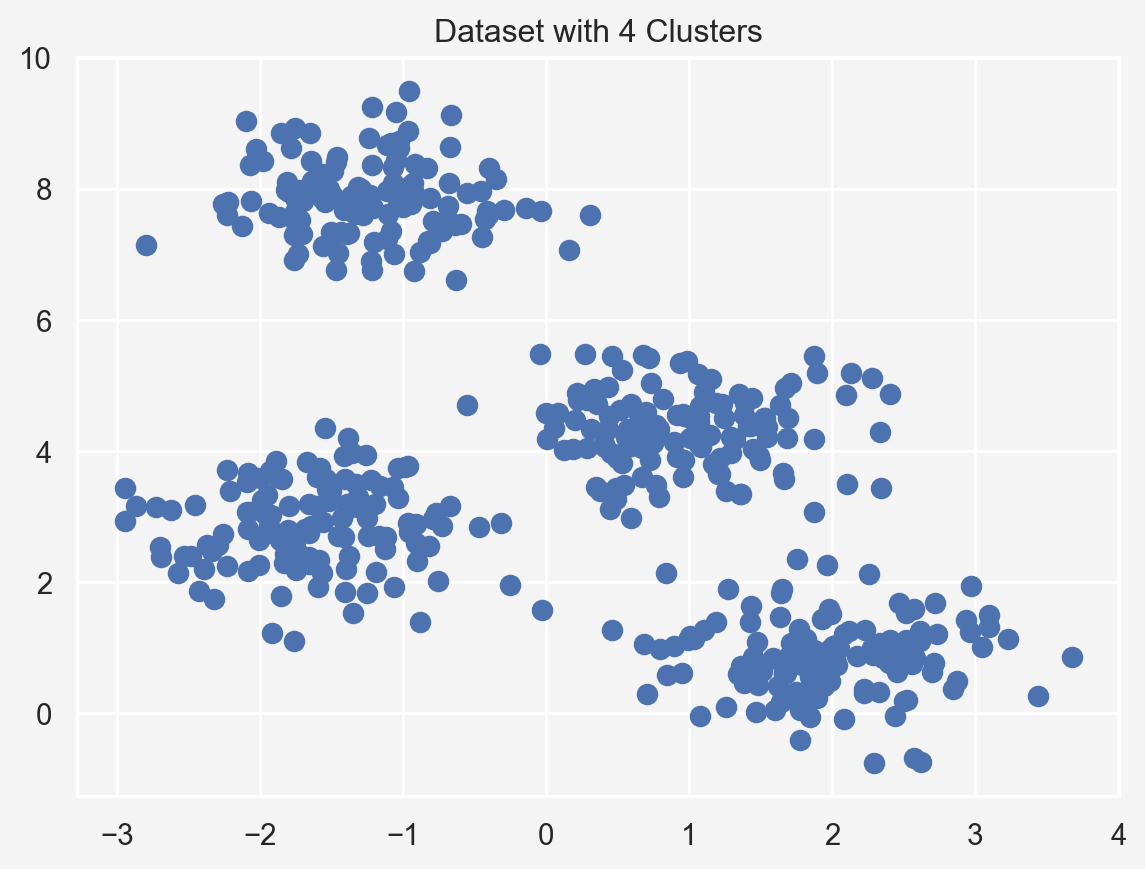
\includegraphics{index_files/figure-pdf/cell-3-output-1.pdf}
\end{center}

We can see from the graph that there appears to be a linear relationship
between the \(x\) and \(y\) values in this case. To find the
relationship mathematically we define the followings

\begin{align*}
S_{xx}& = \sum (x_i-\bar{x})^2 = \sum (x_i^2-2x_i\bar{x}+\bar{x}^2)\\
& = \sum x_i^2 - 2\bar{x}\sum x_i + \sum \bar{x}^2= \sum x_i^2 - 2\bar{x} n \bar{x} + n \bar{x}^2 = \sum x_i ^2 - n \bar{x}^2
\end{align*}

Similarly, \begin{align*}
S_{yy}& = \sum (y_i-\bar{y})^2=\sum y_i ^2 - n \bar{y}^2\\
S_{xy} & = \sum (x_i-\bar{x})^2 \sum (y_i-\bar{y})^2 = \sum x_iy_i -n \bar{xy}
\end{align*}

The sample correlation coefficient \(r\) is then given as

\[
r = \frac{S_{xy}}{\sqrt{S_{xx}S_{yy}}} = \frac{\sum x_i ^2 - n \bar{x}^2}{\sqrt{\left(\sum x_i ^2 - n \bar{x}^2\right)\left(\sum y_i ^2 - n \bar{y}^2\right)}}
\]

You may have seen a different formula to calculate this quantity which
often looks a bit different

\[
\rho = Corr(X,Y)=\frac{Cov(X,Y)}{\sqrt{var(X)var(Y)}}
\]\\
The sample correlation coefficient, \(r\), is an estimator of the
population correlation coefficient, \(\rho\), in the same way as
\(\bar{X}\) is an estimator of \(\mu\) or \(S^2\) is an estimator of
\(\sigma^2\) . Now the question is what does this \(r\) values mean?

\begin{longtable}[]{@{}
  >{\raggedright\arraybackslash}p{(\columnwidth - 2\tabcolsep) * \real{0.3043}}
  >{\raggedright\arraybackslash}p{(\columnwidth - 2\tabcolsep) * \real{0.6957}}@{}}
\toprule\noalign{}
\begin{minipage}[b]{\linewidth}\raggedright
Value
\end{minipage} & \begin{minipage}[b]{\linewidth}\raggedright
Meaning
\end{minipage} \\
\midrule\noalign{}
\endhead
\bottomrule\noalign{}
\endlastfoot
\(r=1\) & The two variables move together in the same direction in a
perfect linear relationship. \\
\(0 < r < 1\) & The two variables tend to move together in the same
direction but there is NOT a direct relationship. \\
\(r= 0\) & The two variables can move in either direction and show no
linear relationship. \\
\(-1 < r < 0\) & The two variables tend to move together in opposite
directions but there is not a direct relationship. \\
\(r =-1\) & The two variables move together in opposite directions in a
perfect linear relationship. \\
\end{longtable}

Let's calculate the correlation of our stock data.

\begin{Shaded}
\begin{Highlighting}[]
\ImportTok{import}\NormalTok{ math}
\NormalTok{x }\OperatorTok{=}\NormalTok{ df.StockPrice.values}
\NormalTok{y }\OperatorTok{=}\NormalTok{ df.Portfolio.values}

\NormalTok{n }\OperatorTok{=} \BuiltInTok{len}\NormalTok{(x)}

\NormalTok{x\_sum, y\_sum }\OperatorTok{=}\DecValTok{0}\NormalTok{,}\DecValTok{0}
\NormalTok{s\_xx, s\_yy, s\_xy }\OperatorTok{=} \DecValTok{0}\NormalTok{,}\DecValTok{0}\NormalTok{,}\DecValTok{0}
\ControlFlowTok{for}\NormalTok{ i }\KeywordTok{in} \BuiltInTok{range}\NormalTok{(n):}
\NormalTok{    x\_sum }\OperatorTok{+=}\NormalTok{ x[i]}
\NormalTok{    s\_xx }\OperatorTok{+=}\NormalTok{ x[i]}\OperatorTok{**}\DecValTok{2}
\NormalTok{    y\_sum }\OperatorTok{+=}\NormalTok{ y[i]}
\NormalTok{    s\_yy }\OperatorTok{+=}\NormalTok{ y[i]}\OperatorTok{**}\DecValTok{2}
\NormalTok{    s\_xy }\OperatorTok{+=}\NormalTok{ x[i]}\OperatorTok{*}\NormalTok{y[i]    }

\NormalTok{s\_xx }\OperatorTok{=}\NormalTok{ s\_xx }\OperatorTok{{-}}\NormalTok{ (x\_sum)}\OperatorTok{**}\DecValTok{2}\OperatorTok{/}\NormalTok{n}
\NormalTok{s\_yy }\OperatorTok{=}\NormalTok{ s\_yy }\OperatorTok{{-}}\NormalTok{ (y\_sum)}\OperatorTok{**}\DecValTok{2}\OperatorTok{/}\NormalTok{n}
\NormalTok{s\_xy }\OperatorTok{=}\NormalTok{ s\_xy }\OperatorTok{{-}}\NormalTok{ (x\_sum }\OperatorTok{*}\NormalTok{ y\_sum)}\OperatorTok{/}\NormalTok{n}

\NormalTok{r }\OperatorTok{=}\NormalTok{ s\_xy}\OperatorTok{/}\NormalTok{math.sqrt(s\_xx }\OperatorTok{*}\NormalTok{ s\_yy)}

\CommentTok{\# Print with formatted labels}
\BuiltInTok{print}\NormalTok{(}\SpecialStringTok{f"Sₓₓ: }\SpecialCharTok{\{}\NormalTok{s\_xx}\SpecialCharTok{:.2f\}}\SpecialStringTok{"}\NormalTok{)}
\BuiltInTok{print}\NormalTok{(}\SpecialStringTok{f"Sᵧᵧ: }\SpecialCharTok{\{}\NormalTok{s\_yy}\SpecialCharTok{:.2f\}}\SpecialStringTok{"}\NormalTok{)}
\BuiltInTok{print}\NormalTok{(}\SpecialStringTok{f"Sₓᵧ: }\SpecialCharTok{\{}\NormalTok{s\_xy}\SpecialCharTok{:.2f\}}\SpecialStringTok{"}\NormalTok{)}
\BuiltInTok{print}\NormalTok{(}\StringTok{\textquotesingle{} \textquotesingle{}}\NormalTok{)}
\BuiltInTok{print}\NormalTok{(}\SpecialStringTok{f"r : }\SpecialCharTok{\{}\NormalTok{r}\SpecialCharTok{:.2f\}}\SpecialStringTok{"}\NormalTok{)}
\end{Highlighting}
\end{Shaded}

\begin{verbatim}
Sₓₓ: 8.53
Sᵧᵧ: 6.97
Sₓᵧ: 7.13
 
r : 0.92
\end{verbatim}

\subsection{Bivariate Analysis}\label{bivariate-analysis}

The joint probability density function for \(X\) and \(Y\) in the
bivariate normal distribution is given by:

\[
f_{X,Y}(x, y) = \frac{1}{2\pi \sigma_X \sigma_Y \sqrt{1-\rho^2}} 
\exp\left( -\frac{1}{2(1-\rho^2)} \left[ \frac{(x-\mu_X)^2}{\sigma_X^2} - 2\rho\frac{(x-\mu_X)(y-\mu_Y)}{\sigma_X \sigma_Y} + \frac{(y-\mu_Y)^2}{\sigma_Y^2} \right] \right)
\]

When \(|\rho| = 1\), the denominator \(\sqrt{1-\rho^2}\) in the PDF
becomes zero, which might appear problematic. However, what happens in
this case is that the joint distribution degenerates into a
\textbf{one-dimensional structure} (a line) rather than being a
two-dimensional probability density.

To see why, consider the quadratic term inside the exponential:

\[
Q = \frac{(x-\mu_X)^2}{\sigma_X^2} - 2\rho \frac{(x-\mu_X)(y-\mu_Y)}{\sigma_X \sigma_Y} + \frac{(y-\mu_Y)^2}{\sigma_Y^2}
\]

When \(|\rho| = 1\), this quadratic expression simplifies, as shown
next.

Start with the simplified \(Q\) when \(|\rho| = 1\):

\begin{align*}
Q &= \left( \frac{x-\mu_X}{\sigma_X} \right)^2 - 2\rho \left( \frac{x-\mu_X}{\sigma_X} \cdot \frac{y-\mu_Y}{\sigma_Y} \right) + \left( \frac{y-\mu_Y}{\sigma_Y} \right)^2\\
&=\left( \frac{x-\mu_X}{\sigma_X} - \rho \frac{y-\mu_Y}{\sigma_Y} \right)^2
\end{align*}

This is a \textbf{perfect square} because the ``cross term'' cancels out
all independent variability of \(X\) and \(Y\) when \(|\rho| = 1\).

For the quadratic term \(Q\) to have any non-zero probability density
(since it appears in the exponent of the PDF), it must be equal to zero:
\[
\frac{x-\mu_X}{\sigma_X} - \rho \frac{y-\mu_Y}{\sigma_Y} = 0
\]

Rearranging this equation: \[
\frac{y-\mu_Y}{\sigma_Y} = \rho \frac{x-\mu_X}{\sigma_X}
\]

Multiply through by \(\sigma_Y\): \[
y - \mu_Y = \rho \frac{\sigma_Y}{\sigma_X} (x - \mu_X)
\]

Thus: \[
y = \mu_Y + \rho \frac{\sigma_Y}{\sigma_X} (x - \mu_X)
\]

This is the equation of a straight line in the \((X, Y)\)-plane. The
slope of the line is \(\rho \frac{\sigma_Y}{\sigma_X}\), and the line
passes through the point \((\mu_X, \mu_Y)\). When \(|\rho| = 1\), all
the joint probability mass collapses onto this line, meaning \(X\) and
\(Y\) are perfectly linearly dependent.

\begin{Shaded}
\begin{Highlighting}[]
\NormalTok{// Import necessary libraries}
\NormalTok{Plot = require(\textquotesingle{}@observablehq/plot\textquotesingle{})}
\NormalTok{d3 = require(\textquotesingle{}d3@7\textquotesingle{})}

\NormalTok{// Define the bivariate normal PDF function}
\NormalTok{function bivariateNormalPDF(x, y, muX, muY, sigmaX, sigmaY, rho) \{}
\NormalTok{  const z =}
\NormalTok{    ((x {-} muX) ** 2) / sigmaX ** 2 {-}}
\NormalTok{    (2 * rho * (x {-} muX) * (y {-} muY)) / (sigmaX * sigmaY) +}
\NormalTok{    ((y {-} muY) ** 2) / sigmaY ** 2;}
\NormalTok{  const denominator = 2 * Math.PI * sigmaX * sigmaY * Math.sqrt(1 {-} rho ** 2);}
\NormalTok{  return Math.exp({-}z / (2 * (1 {-} rho ** 2))) / denominator;}
\NormalTok{\}}

\NormalTok{// Parameters}
\NormalTok{const muX = 0,}
\NormalTok{  muY = 0,}
\NormalTok{  sigmaX = 1,}
\NormalTok{  sigmaY = 1;}

\NormalTok{// Create a slider for rho}
\NormalTok{viewof rho = Inputs.range([{-}0.99, 0.99], \{ step: 0.01, value: 0, label: \textquotesingle{}Correlation (ρ)\textquotesingle{} \})}

\NormalTok{// Generate grid data}
\NormalTok{const x = d3.range({-}3, 3.1, 0.1);}
\NormalTok{const y = d3.range({-}3, 3.1, 0.1);}
\NormalTok{const grid = x.flatMap((xi) =\textgreater{} y.map((yi) =\textgreater{} (\{ x: xi, y: yi, z: bivariateNormalPDF(xi, yi, muX, muY, sigmaX, sigmaY, rho) \})));}

\NormalTok{// Create the contour plot}
\NormalTok{Plot.plot(\{}
\NormalTok{  marks: [}
\NormalTok{    Plot.contour(grid, \{}
\NormalTok{      x: \textquotesingle{}x\textquotesingle{},}
\NormalTok{      y: \textquotesingle{}y\textquotesingle{},}
\NormalTok{      z: \textquotesingle{}z\textquotesingle{},}
\NormalTok{      stroke: \textquotesingle{}steelblue\textquotesingle{},}
\NormalTok{      strokeWidth: 1,}
\NormalTok{      thresholds: 10,}
\NormalTok{    \}),}
\NormalTok{  ],}
\NormalTok{  x: \{}
\NormalTok{    label: \textquotesingle{}X\textquotesingle{},}
\NormalTok{  \},}
\NormalTok{  y: \{}
\NormalTok{    label: \textquotesingle{}Y\textquotesingle{},}
\NormalTok{  \},}
\NormalTok{  color: \{}
\NormalTok{    legend: true,}
\NormalTok{    label: \textquotesingle{}Density\textquotesingle{},}
\NormalTok{  \},}
\NormalTok{  width: 600,}
\NormalTok{  height: 600,}
\NormalTok{\})}
\end{Highlighting}
\end{Shaded}



\printbibliography



\end{document}
